% CREATED BY DAVID FRISK, 2016
\chapter{Results}
\section{Experiment 1: Baseline Evaluation \& Blindfolding}
Fig.~\ref{fig:training_metrics} shows metrics for each batch during training. Fig.~\ref{fig:baseline_metrics} shows metrics averaged for each epoch during the baseline evaluation. Fig.~\ref{fig:blindfolded_metrics} shows metrics averaged for each epoch during blindfolded evaluation. It's clear in this graphs that the evaluation results are more stable when the model is given images. As can be seen in Figures~\ref{fig:baseline_loss} \& ~\ref{fig:blindfolded_loss}, the model begins to overfit to the training data around epoch 10. 
Table~\ref{tab:best_baseline} shows the checkpoints with lowest loss, highest accuracy, and lowest mean rank during the evaluation of the baseline, with the metric that was "best" during that checkpoint in bold. Table~\ref{tab:best_blindfolded} shows the same for blindfolded evaluation. Comparing their best, the blindfolded model has 4.7\% worse loss than the baseline, 0.212 higher loss, and 0.149 higher mean rank. 

\begin{figure}
     \centering
     \begin{subfigure}[b]{0.3\textwidth}
         \centering
         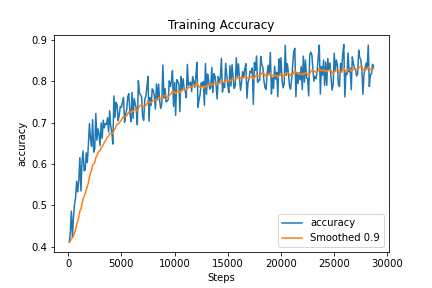
\includegraphics[width=\textwidth]{/home/yasmeen/Desktop/thesisproj/thesis/figure/results/baseline_and_blindfolding/training/accuracy.png}
         \caption{Training Accuracy}
         \label{fig:training_accuracy}
     \end{subfigure}
     \hfill
     \begin{subfigure}[b]{0.3\textwidth}
         \centering
         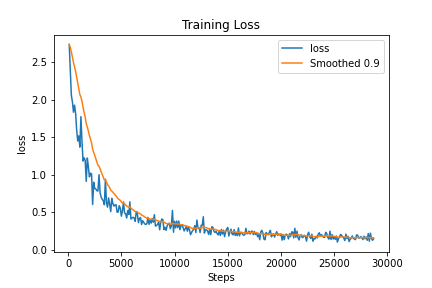
\includegraphics[width=\textwidth]{/home/yasmeen/Desktop/thesisproj/thesis/figure/results/baseline_and_blindfolding/training/loss.png}
         \caption{Training Loss}
         \label{fig:training_loss}
     \end{subfigure}
     \hfill
     \begin{subfigure}[b]{0.3\textwidth}
         \centering
         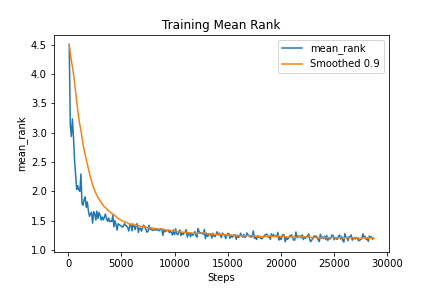
\includegraphics[width=\textwidth]{/home/yasmeen/Desktop/thesisproj/thesis/figure/results/baseline_and_blindfolding/training/mean_rank.png}
         \caption{Training Mean Rank}
         \label{fig:training_mean_rank}
     \end{subfigure}
     \caption{Training Metrics}
     \label{fig:training_metrics}
\end{figure}

\begin{figure}
     \centering
     \begin{subfigure}[b]{0.3\textwidth}
         \centering
         \includegraphics[width=\textwidth]{/home/yasmeen/Desktop/thesisproj/thesis/figure/results/baseline_and_blindfolding/images/avg val accuracy.png}
         \caption{Baseline Validation Accuracy}
         \label{fig:baseline_accuracy}
     \end{subfigure}
     \hfill
     \begin{subfigure}[b]{0.3\textwidth}
         \centering
         \includegraphics[width=\textwidth]{/home/yasmeen/Desktop/thesisproj/thesis/figure/results/baseline_and_blindfolding/images/avg val loss.png}
         \caption{Baseline Validation Loss}
         \label{fig:baseline_loss}
     \end{subfigure}
     \hfill
     \begin{subfigure}[b]{0.3\textwidth}
         \centering
         \includegraphics[width=\textwidth]{/home/yasmeen/Desktop/thesisproj/thesis/figure/results/baseline_and_blindfolding/images/avg val mean rank.png}
         \caption{Baseline Validation Mean Rank}
         \label{fig:baseline_mean_rank}
     \end{subfigure}
     \caption{Baseline Validation Metrics}
     \label{fig:baseline_metrics}
\end{figure}


\begin{figure}
     \centering
     \begin{subfigure}[b]{0.3\textwidth}
         \centering
         \includegraphics[width=\textwidth]{/home/yasmeen/Desktop/thesisproj/thesis/figure/results/baseline_and_blindfolding/blindfolded/avg val accuracy.png}
         \caption{Blindfolded Validation Accuracy}
         \label{fig:blindfolded_accuracy}
     \end{subfigure}
     \hfill
     \begin{subfigure}[b]{0.3\textwidth}
         \centering
         \includegraphics[width=\textwidth]{/home/yasmeen/Desktop/thesisproj/thesis/figure/results/baseline_and_blindfolding/blindfolded/avg val loss.png}
         \caption{Blindfolded Validation Loss}
         \label{fig:blindfolded_loss}
     \end{subfigure}
     \hfill
     \begin{subfigure}[b]{0.3\textwidth}
         \centering
         \includegraphics[width=\textwidth]{/home/yasmeen/Desktop/thesisproj/thesis/figure/results/baseline_and_blindfolding/blindfolded/avg val mean rank.png}
         \caption{Blindfolded Validation Mean Rank}
         \label{fig:blindfolded_mean_rank}
     \end{subfigure}
     \caption{Blindfolded Validation Metrics}
     \label{fig:blindfolded_metrics}
\end{figure}

\begin{table}[h]
\centering
\caption{"Best" Epochs During Baseline Evaluation}
\begin{tabular}{l | l | l | l}
Checkpoint & Loss & Accuracy & Mean Rank \\
\hline
8 & \textbf{2.204141} & 0.381122 & 4.341837 \\
15 & 2.404433 & \textbf{0.403061} & 4.138265 \\
23 & 2.691763 & 0.370408 & \textbf{4.110714}
\end{tabular}
\label{tab:best_baseline}
\end{table}

\begin{table}[h]
\centering
\caption{"Best" Epochs During Blindfolded Evaluation}
\begin{tabular}{l | l | l | l}
Checkpoint & Loss & Accuracy & Mean Rank \\
\hline
5 & \textbf{2.416477} & 0.246429 & 5.493877 \\
27 & 2.546098 & \textbf{0.355612} & 4.551021 \\
39 & 4.788071 & 0.307653 & \textbf{4.260204}
\end{tabular}
\label{tab:best_blindfolded}
\end{table}


